\chapter{Netzwerk-Spiel}\label{sec:netzwerkspiel}
\begin{figure}[H]
    \centering
    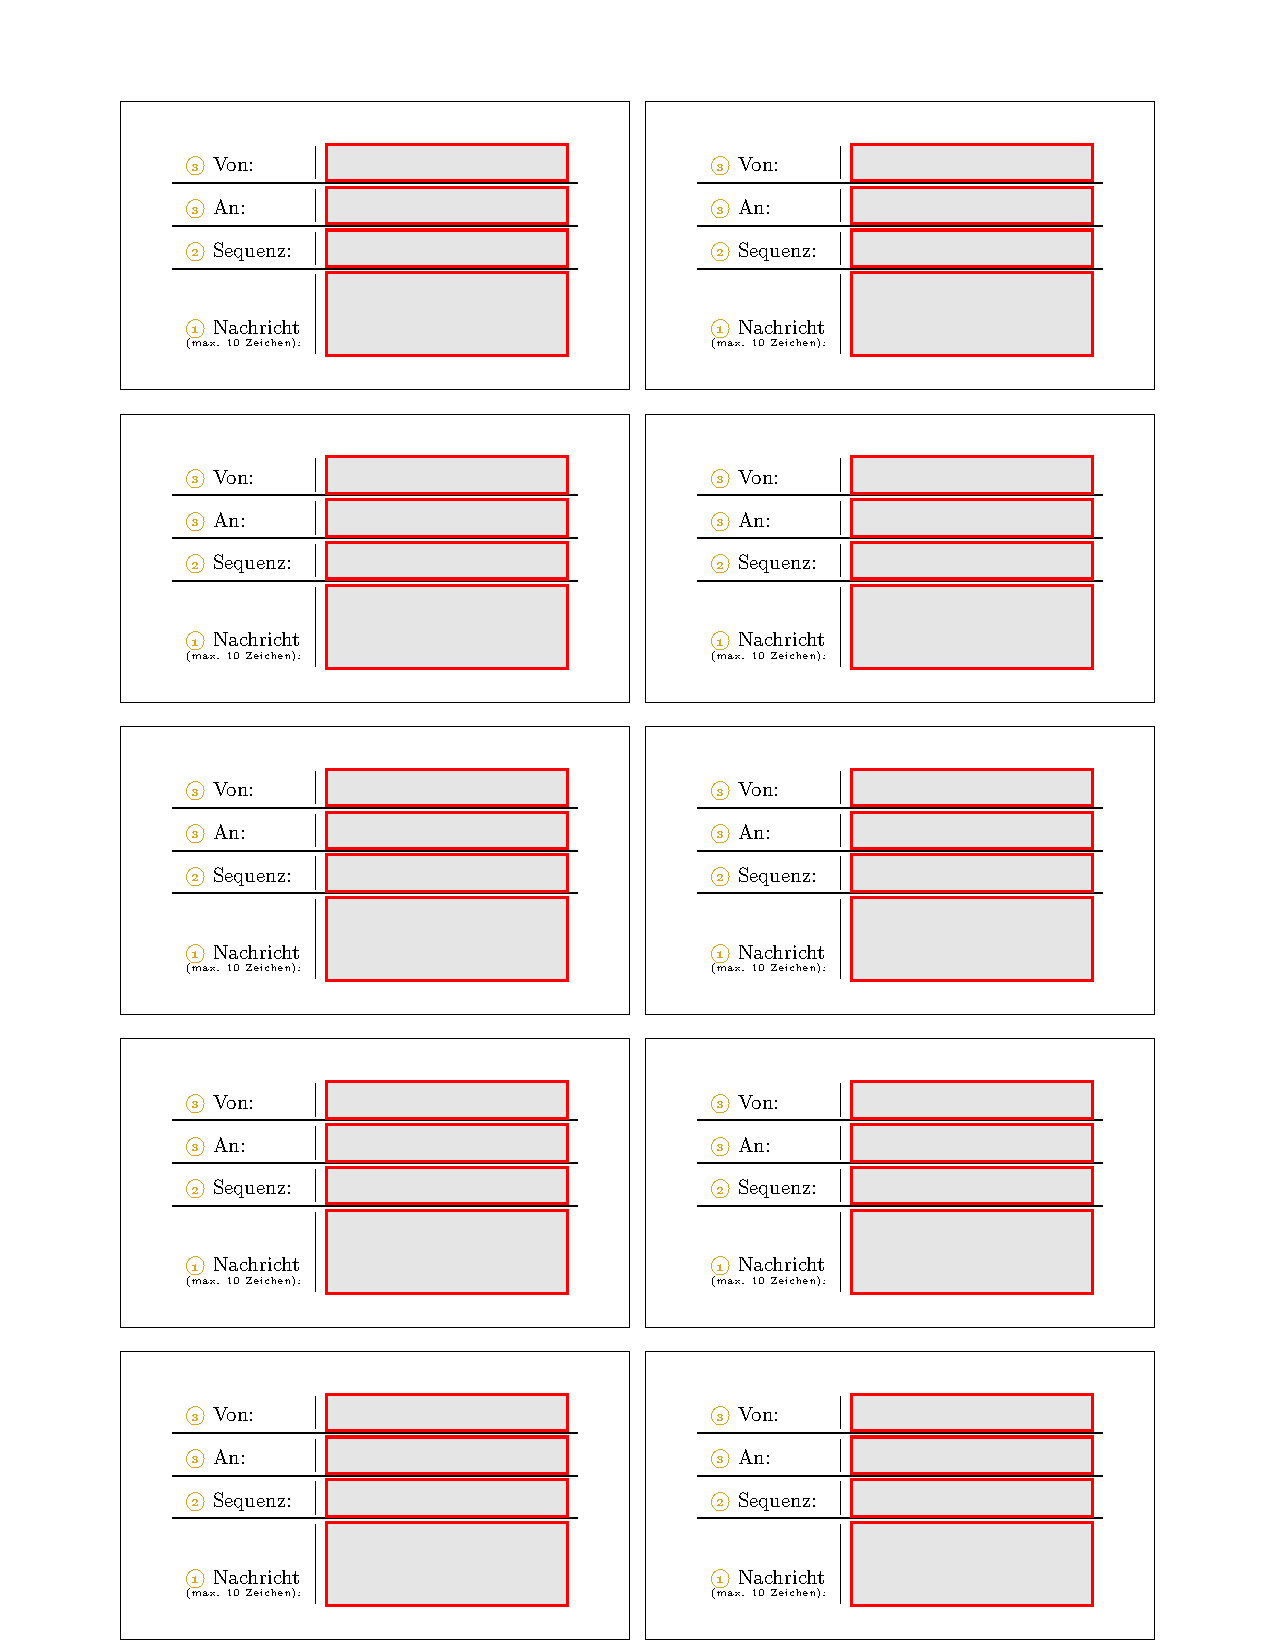
\includegraphics[width=.7\textwidth]{Grundlagen_Info/07_Netzwerke/Skript/Zettel.pdf}
    \caption{Zettel für das Netzwerk-Spiel}
\end{figure}
\clearpage

In dieser Übung sollen Sie die verschiedenen Schichten des Netzwerk-Schichtenmodells anhand eines praktischen Beispiels anwenden. Dabei schicken Sie sich gegenseitig Nachrichten zu, indem sie die IP-Adresse der anderen Person verwenden. Die IP-Adresse wurde im Vorfeld von der Lehrperson zugeteilt, welche ebenfalls die Rolle des Routers (innerhalb eines lokalen Netzwerks) übernimmt. Das Spiel läuft wie folgt ab:

\begin{enumerate}
	\item Jede Person erhält ein ausgedrucktes Namensschild mit dazugehöriger IP-Adresse. Das Namensschild wird so platziert, dass es für alle gut sichtbar ist.
	\item Die Lehrperson erklärt die verschiedenen Schichten des Netzwerk-Schichtenmodells und wie sie in diesem Spiel angewendet werden.
	\item Jede Person schreibt eine kurze Nachricht (z.B. ``Hallo, wie geht's?'') und adressiert sie an eine andere Person, indem sie deren IP-Adresse verwendet. Die maximale Nachrichtenlänge beträgt 10 Zeichen.
	\item Die Nachricht wird mit einer Sequenznummer versehen, um die Reihenfolge der Nachrichten zu kennzeichnen (Couvert Grösse \texttt{A6}).
	\item  Die Nachricht wird in ein Couvert gesteckt, welches die IP-Adresse des Empfängers auf der Vorderseite und die eigene IP-Adresse auf der Rückseite trägt (Couvert Grösse \texttt{A5}).
	\item Die Lehrperson fungiert als Router und sammelt die Couvert-Nachrichten. Sie überprüft, ob die IP-Adressen korrekt sind und ob die Nachrichten an die richtige Person adressiert sind.
	\item Die Lehrperson verteilt die Couvert-Nachrichten an die entsprechenden Empfänger, indem sie die IP-Adressen auf den Couvert-Nachrichten überprüft.
	\item Die Empfänger öffnen die Couvert-Nachrichten und sortieren die Nachrichten nach Sequenz-Nummer. Sie lesen die Nachrichten laut vor und beantworten sie gegebenenfalls.
	\item Die Lehrperson fasst die Übung zusammen und erklärt, wie das Netzwerk-Schichtenmodell in der Praxis funktioniert. Dabei wird auf die verschiedenen Schichten eingegangen und erläutert, wie sie in diesem Spiel umgesetzt wurden.
	\item Optional: Die Lehrperson kann die Übung erweitern, indem sie verschiedene Netzwerk-Szenarien simuliert, z.B. Netzwerk-Ausfälle, Verzögerungen oder Störungen, um die Auswirkungen auf die Kommunikation zu verdeutlichen.
	\item Mögliche Erweiterung des Spiels: zweiter und dritter Router (Personen) bestimmen, um die Konzepte von Subnetzen und Routing zu verdeutlichen. Konzepte: Netzmaske, Gateway, Interface, Routing-Tabelle.
\end{enumerate}